\chapter{Projekt aplikacji}

W ramach części praktycznie pracy wykonano aplikację internetową \mbox{\textit{ProjectSHARE}}. Podczas implementacji skupiono się głównie nad stworzeniem prostego, wygodnego interfejsu użytkownika oraz nad dostosowaniem wyświetlanej treści do użytkownika. Aby osiągnąć zamierzone rezultaty, w procesie wytwarzania aplikacji wykorzystano metodologię zwinną oraz związane z nią krótkie iteracje, ustalenie wymagań na podstawie tzw. \textit{User Stories} oraz estymację kosztów wytworzenia funkcjonalności za pomocą techniki \textit{Planning Poker}.

\section{Założenia}

Główne założenia towarzyszące projektowaniu aplikacji to: prostota interfejsu
użytkownika, łatwe wyszukiwanie projektów, rekomendacja projektów wykorzystująca informacje o użytkowniku oraz odgórne
ograniczenie ilości udostępnianych informacji o projekcie. Część aplikacji wzorowana jest na kilku
rozwiązaniach wykorzystywanych w bardzo popularnych serwisach, np. ograniczona liczba
znaków stosowana w aplikacji Twitter oraz prosta mechanika oznaczania jako obserwowane. W systemie
rekomendacji wykorzystywany jest algorytm uczenia Content-based filtering, który na podstawie tagów projektów oznaczonych jako obserwowane, wyszuka w bazie danych odpowiednie przedsięwzięcia.

Wyżej wymienione założenia pozwalają na stworzenie platformy nadającej się dla
każdego, ponieważ wyświetlane projekty są dostosowane do użytkownika. Dodatkowo autor ukrywa całą implementacje i szczegóły
swojej pracy, ponieważ istnieje odgórne ograniczenie znaków w opisie projektu. Dzięki temu
założeniu możliwa jest również współpraca bezpośrednio z przedsiębiorstwami, które mogą udostępnić
jedynie ogólny opis swojego produktu. Daje to dodatkowe możliwości takie jak np.
darmowa reklama lub rekrutacja innych użytkowników. Jednocześnie
branża w której autor się obraca nie ma tak wielkiego znaczenia jak w przypadku innych
repozytorium, ponieważ projekty oznaczane są odpowiednimi tagami, a serwis wyszukuje
je wedle upodobań autora.

\bigskip
\bigskip
\bigskip
\bigskip

\section{Specyfikacja wymagań}

Wymagania zostały podzielone na dwie kategorie: biznesowe oraz technicznie. Biznesowe oznaczają wymaganie sprecyzowane przez klienta w postaci historyjek użytkownika. Są one krótkim opisem cech i właściwości systemu z perspektywy potrzeb użytkownika. Mają one ujednoliconą strukturę w postaci ,,Jako ... chcę ..., ponieważ ...''.  Ustala się je we współpracy z klientem tak, aby uwzględnić w nich najważniejsze aspekty np. łatwość oszacowania kosztu wytworzenia, wartość biznesowa, określenie kryteriów akceptacji, możliwość wykonania w obrębie jednej iteracji. Ich największą zaletą jest uspójnienie wizji, określenie pożądanego efektu oraz minimalizacja ryzyka wystąpienia nieporozumienia. Techniczne wymagania są natomiast ustalane przez zespół programistów na podstawie wymagań biznesowych. Z reguły nie są one prezentowane klientowi, ponieważ są one zrozumiałe dla konkretnej grupy osób. Ich zadaniem jest określenie konkretnych elementów systemu, które należy wykonać. W przypadku metodyki agile powinny one być uzupełnieniem wymagań biznesowych oraz podlegać ciągłej zmianie \cite{AGI01}. Ich niewątpliwą zaletą jest możliwość pokazania większej abstrakcji systemu, niż w przypadku historyjki użytkownika. Jedno wymaganie techniczne może odnosić się do kilku scenariuszy wynikających z historyjek biznesowych, dzięki czemu koszt jest mocno redukowany. Inną zaletą ich stosowania jest większa przejrzystość dla programisty. 

\bigskip

Dla aplikacji \mbox{\textit{ProjectSHARE}} wyróżniono następujące wymagania biznesowe w postaci \textit{User Stories}:
\begin{itemize}
	\item[$\bullet$] Jako użytkownik chciałbym mieć możliwość logowania za pomocą adresu e-mail, ponieważ jest to wygodny standard w wielu aplikacjach internetowych
	\item[$\bullet$] Jako użytkownik chciałbym mieć możliwość tworzenia inicjatyw publicznych oraz łączenia się w zespoły, ponieważ znalezienie osób chętnych do realizacji projektu jest dzięki temu prostsze i szybsze
	\item[$\bullet$] Jako użytkownik chciałbym mieć możliwość tworzenia inicjatyw prywatnych, tak abym mógł sam zdecydować, kto dołączy do projektu 
	\item[$\bullet$] Jako użytkownik chciałbym móc wysyłać zaproszenia do konkretnych użytkowników, tak aby mogli dołączyć do projektu prywatnego
	\item[$\bullet$] Jako użytkownik chciałbym, aby wyświetlały mi się projekty dostosowane do moich zainteresowań, ponieważ zaoszczędzę w ten sposób czas spędzony na szukaniu interesujących projektów
	\item[$\bullet$] Jako użytkownik chciałbym mieć możliwość wygodnego przeglądania innych projektów
	\item[$\bullet$] Jako użytkownik chciałbym oznaczyć projekt jako obserwowany, ponieważ będę miał możliwość szybkiego powrotu do niego
	\item[$\bullet$] Jako użytkownik chciałbym mieć możliwość komunikacji z innym użytkownikiem, ponieważ wymiana informacji jest jednym z kluczowych aspektów przy pracy w projekcie oraz przy rekrutacji innych użytkowników do projektu
	\item[$\bullet$] Jako użytkownik chciałbym, aby powiadomienia przychodziły mi na maila, ponieważ mógłbym zostać powiadomiony o jakiejś akcji bez wchodzenia do aplikacji
	\item[$\bullet$] Jako użytkownik chciałbym móc przeglądać profil innego użytkownika, ponieważ daje mi to możliwość weryfikacji jego aktualnych działań oraz projektów
	\item[$\bullet$] Jako użytkownik chciałbym móc wyszukać projekt po tagach, ponieważ jest to bardziej precyzyjne.
\end{itemize}

\bigskip

Na podstawie wymagań biznesowych wyróżniono następujące wymagania techniczne w postaci elementów systemu:
\begin{itemize}
	\item[$\bullet$] Panel logowania za pomocą email
	\item[$\bullet$] Formularz rejestracji
	\item[$\bullet$] Panel służący do wyświetlania profilu użytkownika
	\item[$\bullet$] Panel wyświetlający rekomendowane projekty
	\item[$\bullet$] Panel wyświetlający listę projektów obserwowanych
	\item[$\bullet$] Komunikator
	\item[$\bullet$] Panel z informacjami o projekcie
	\item[$\bullet$] Formularz tworzenia projektu
	\item[$\bullet$] Wyszukiwarka projektów
	\item[$\bullet$] Algorytm Content-based filtering dla systemu rekomendacji
	\item[$\bullet$] Powiadomienia email
\end{itemize}

\section{Realizacja aplikacji}

Proces implementacji został podzielony na 4 dwutygodniowe iteracje. Ilość iteracji była ograniczona przez ustalony z góry termin osiągnięcia tzw. produktu o minimalnej wartości. Aplikacja spełnia założenia tego typu produktu w przypadku, gdy oferuje najważniejsze funkcjonalności określone przez klienta. Aby to osiągnąć przeprowadzono najpierw estymację kosztu wyprodukowania wszystkich historyjek użytkownika za pomocą techniki \textit{Planning Poker}. Wartości przydzielane poszczególnym historyjką zostały ustalone za pomocą kolejnych liczb ciągu Fibonacciego. Jako zdolność zespołu na każdą iterację przyjęto wartość 30, co również służyło jako punkt odniesienia podczas estymacji kosztów. Poniżej znajduje się tabela zawierająca skrócony opis wszystkich historyjek oraz przydzielone do nich \textit{story points}.


\begin{figure}[h!]
	\makebox[\textwidth][c]{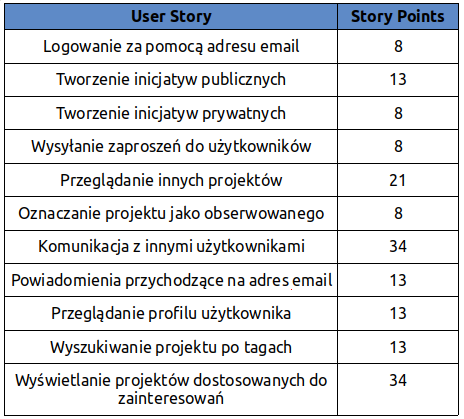
\includegraphics[scale=0.6]{UserStories}
	}
	\caption{Tabela historyjek użytkownika wraz z przydzielonymi punktami}
	\centering
\end{figure}

Suma wszystkich punktów wynosi 173. Biorąc pod uwagę zdolność zespołu oraz liczbę iteracji możliwe jest spełnienie tylko 120 punktów, dlatego w następnym kroku określono historyjki najważniejsze z punktu widzenia klienta. Mając te dane przystąpiono do planowania poszczególnych iteracji oraz historyjek które mają zostać zaimplementowane w każdej z nich. Tak powstały plan był głównym artefaktem podczas procesu implementacji, który jasno wyznaczał jakie zadanie mają zostać spełnione w danej iteracji. Zgodne z metodologią zwinną ulegał on pewnym zmianą wraz z postępami oraz zmieniającymi się wymaganiami co jest, jednak przez dobre oszacowanie kosztów zmiany były nieznaczne. 
\bigskip

\begin{figure}[h!]
	\makebox[\textwidth][c]{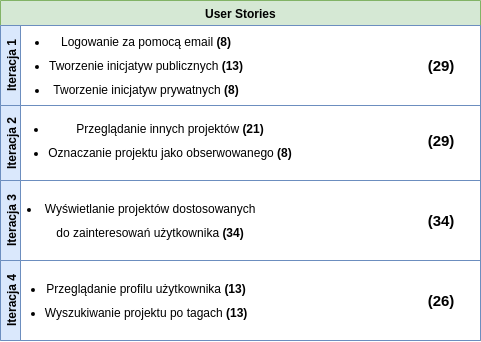
\includegraphics[scale=0.6]{Iteracje}
	}
	\caption{Iteracje wraz z przydzielonymi historyjkami}
	\centering
\end{figure}

\section{Model bazy danych}
Struktura bazy danych została zaprojektowana tak, aby implementacja założonych  funkcjonalności była jak najprostsza. Jest ona jednocześnie zwarta i przejrzysta, co pozwala na dalszą jej rozbudowę oraz dodanie nowych tabel w przypadku potrzeby implementacji nowej funkcjonalności. Poniżej znajduje się diagram ERD przedstawiający zależności między tabelami.
\begin{figure}[h!]
	\makebox[\textwidth][c]{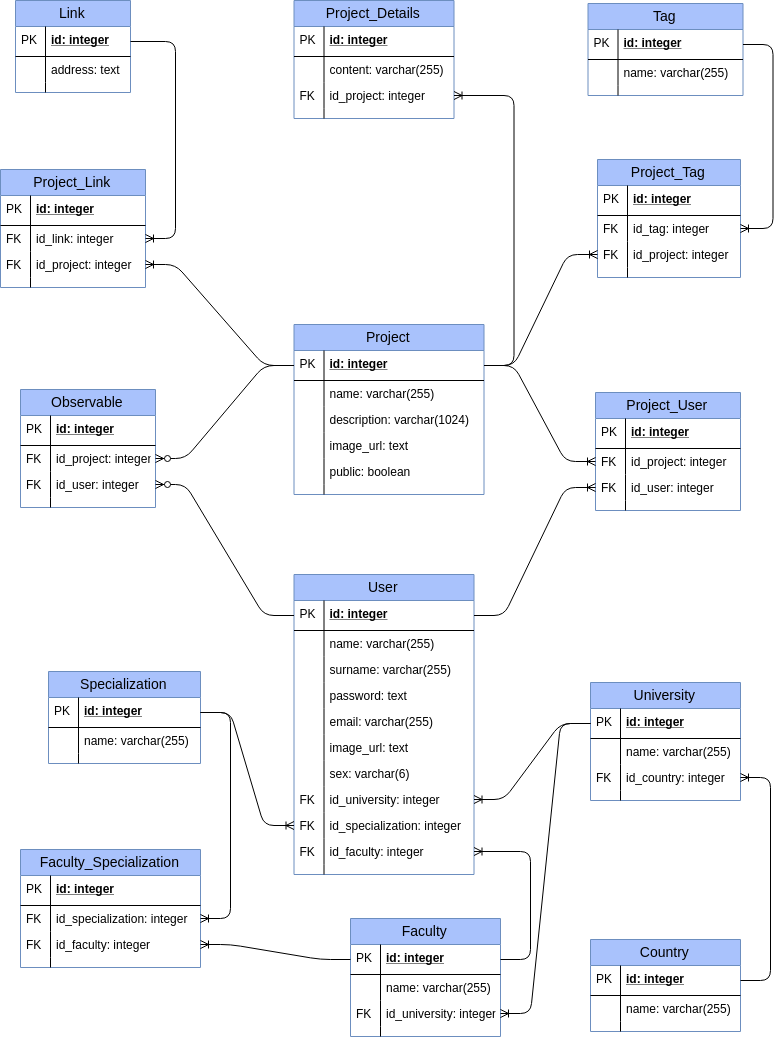
\includegraphics[scale=0.5]{Database}
	}
	\caption{Diagram ERD bazy danych}
	\centering
\end{figure}


\section{Architektura systemu}

Aplikacja składa się z 3 głównych elementów: bazy danych, warstwy back-end w postaci Representational State Transfer Application Programming Interface oraz aplikacji internetowej typu Single Page. Każdy z wyżej wymienionych elementów stanowi osobną całość w systemie, co pozwala na niezależne rozwijanie każdej z nich. Najniższą warstwa to warstwa bazy danych, która jest odpowiedzialna za przechowywanie informacji. Do zarządzania bazą danych oraz zasobami służy REST API, które udostępnia wybrane operację poprzez protokół HTTP. Każdy zasób posiada unikalną ścieżkę, dzięki której można się do niego odwołać oraz wykonać operacje Create, Read, Update, Delete. Udostępniane dane są w formacie JavaScript Object Notation. W przypadku tworzenia danego zasobu, dane potrzebne do stworzenia obiektu również są w formacie JSON. Elementem systemu służącym jako interfejs użytkownika jest aplikacja internetowa typu Single Page, która pozwala na interakcję użytkownika z systemem bez opóźnień wynikających z przeładowania strony. Opiera się na asynchronicznej komunikacji z wspomnianym wyżej REST API. Dodatkowo separuje logikę związaną z wyświetlaniem informacji użytkownikowi.
\bigskip

\begin{figure}[h!]
	\makebox[\textwidth][c]{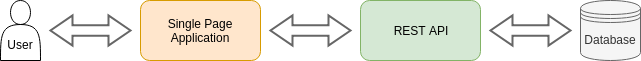
\includegraphics[scale=0.6]{SimpleArchitecture}
	}
	\caption{Uproszczona architektura systemu}
	\centering
\end{figure}

\bigskip

\subsection{Struktura REST API}

REST API do wykonania operacji na odpowiednim zasobie wykorzystuje strukturę drzewiastą, która jest reprezentowana przez ścieżki URL. Zgodnie z przyjętą konwencją, każdy punkt końcowy reprezentuje zasób jako rzeczownik w liczbie mnogiej. Aby dostać się do niego należy wysłać odpowiednie żądanie. Jeżeli jest ono prawidłowe, w odpowiedzi przesyłany jest najczęściej obiekt w formacie JSON reprezentujący zasób oraz kod statusu HTTP. Do poszczególnych zasobów powinno się odwoływać od najbardziej ogólnego elementu do najbardziej szczegółowego. Dla każdej ścieżki mogą zostać zaimplementowane cztery metody HTTP: GET, POST, PUT, DELETE. Reprezentują one operację typu CRUD, które można wykonać na danym zasobie. Dodatkowo można zdefiniować, które parametry HTTP Headers są wymagane w żądaniu, co pozwala na zabezpieczenie dostępu do zasobu poprzez np. autoryzację za pomocą tokenów. Poniżej znajdują się diagramy reprezentujące zaimplementowane punkty końcowe ścieżki dla aplikacji \mbox{\textit{ProjectSHARE}} wraz z możliwymi operacjami.

\bigskip
\bigskip
\bigskip
\bigskip
\bigskip
\bigskip
\bigskip
\bigskip
\bigskip
\bigskip
\bigskip\bigskip
\bigskip\bigskip
\bigskip\bigskip
\bigskip\bigskip
\bigskip


\begin{figure}[h!]
	\makebox[\textwidth][c]{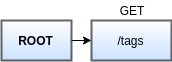
\includegraphics[scale=0.6]{TagsEndpoints}
	}
	\caption{Ścieżki URL do wykonania operacji na tagach}
	\centering
\end{figure}



\begin{figure}[h!]
	\makebox[\textwidth][c]{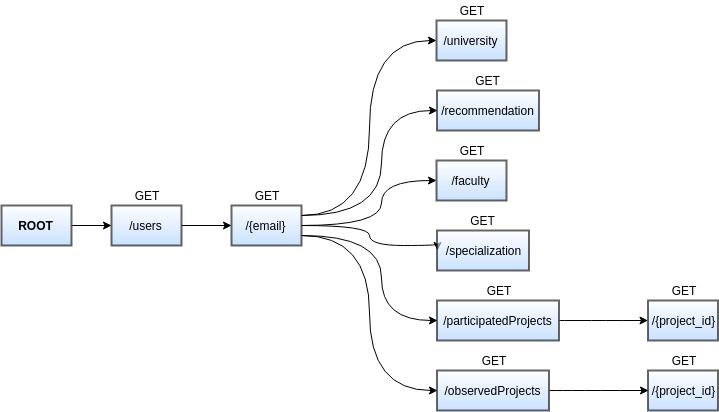
\includegraphics[scale=0.55]{UserEndpoints}
	}
	\caption{Ścieżki URL do wykonania operacji na użytkownikach}
	\centering
\end{figure}


\begin{figure}[h!]
	\makebox[\textwidth][c]{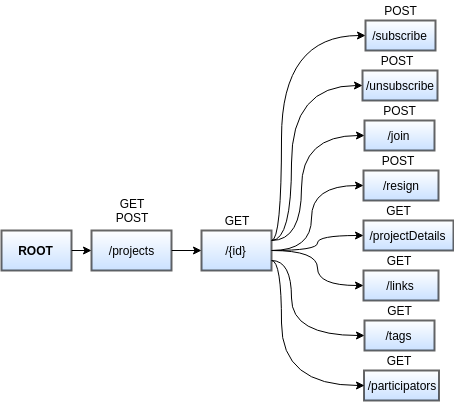
\includegraphics[scale=0.6]{ProjectsEndpoints}
	}
	\caption{Ścieżki URL do wykonania operacji na projektach}
	\centering
\end{figure}


\begin{figure}[h!]
	\makebox[\textwidth][c]{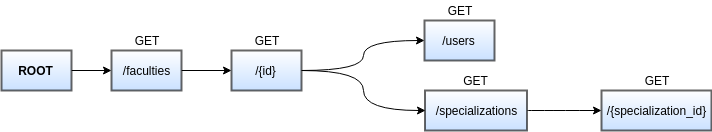
\includegraphics[scale=0.5]{FacultiesEndpoints}
	}
	\caption{Ścieżki URL do wykonania operacji na wydziałach}
	\centering
\end{figure}

\begin{figure}[h!]
	\makebox[\textwidth][c]{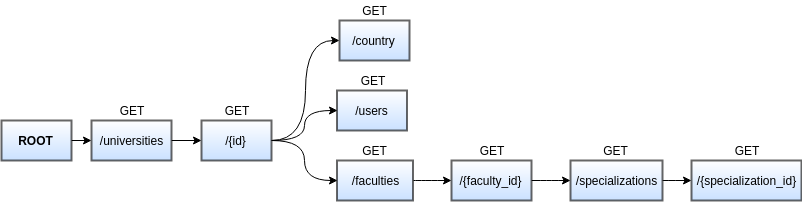
\includegraphics[scale=0.5]{UniversitiesEndpoints}
	}
	\caption{Ścieżki URL do wykonania operacji na uniwersytetach}
	\centering
\end{figure}

\begin{figure}[h!]
	\makebox[\textwidth][c]{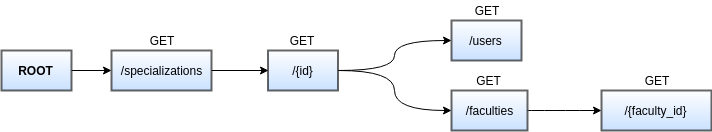
\includegraphics[scale=0.5]{SpecializationsEndpoints}
	}
	\caption{Ścieżki URL do wykonania operacji na specjalizacjach}
	\centering
\end{figure}





\subsection{Architektura aplikacji internetowej}

Aplikacja internetowa \mbox{\textit{ProjectSHARE}} składa się z kilku komponentów wydzielających logikę związaną z konkretną funkcjonalnością. Każdy komponent jest dynamicznie wstrzykiwany w zależności od przypisanej do niego ścieżki URL, co zwiększa wydajność aplikacji oraz poprawia komfort użytkowania. Za poruszanie się po ścieżkach oraz dobór odpowiednich komponentów odpowiedzialny jest specjalny \textit{router}, będący wbudowanym narzędziem szkieletu Angular. Informację o tym, który komponent jest przypisany do jakiej ścieżki oraz czy może zostać w danym momencie wyświetlony są przechowywane w wydzielonym module \textit{app-route}. Za komunikację z REST API odpowiedzialne są następujące serwisy: \textit{UserService, ProjectService, TagService, UserAuthService}. Każdy serwis oznaczone adnotacją \textit{@Injectable()} może zostać wstrzyknięty do komponentu poprzez konstruktor. Ich głównym zadaniem jest implementacja odpowiednich metod wywołujący określone operacje na zasobach REST API. Serwisy te również przekazują asynchronicznie dane do konkretnych komponentów korzystając z modelu komunikacji Publisher-Subscriber. Dodatkowo istnieje jeszcze jeden serwis \textit{AuthGuardService} implementujący interfejs \textit{CanActivate}. Pozwala on na zdefiniowanie metody zwracającej informację o tym, czy dany komponent może zostać wyświetlony w zależności od tego, czy użytkownik jest zalogowany czy też nie. Jest on stosowany tylko we wspomnianym wyżej wymienionym module \textit{app-route}.

\begin{figure}[h!]
	\makebox[\textwidth][c]{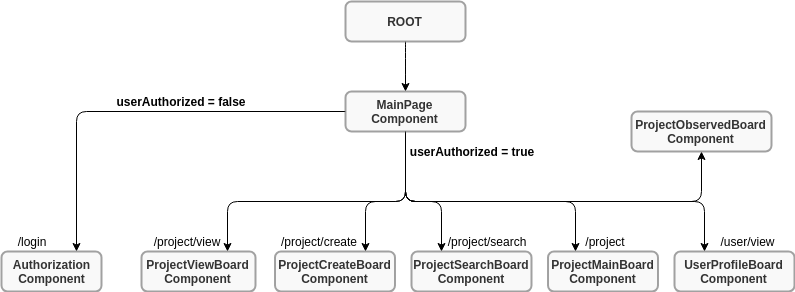
\includegraphics[scale=0.5]{SPAStructure}
	}
	\caption{Struktura komponentów wraz z odpowiadającymi im ścieżkami}
	\centering
\end{figure}


\section{Interfejs użytkownika}

Podczas projektowania interfejsu użytkownika kierowano się głównie wygodą interakcji użytkownika z aplikacją oraz starano się stworzyć go jasnym i przejrzystym. Wzorowano się na najpopularniejszych serwisach dostępnych w internecie oraz stylu projektowania aplikacji internetowych o nazwie \textit{Material Design}. Do wygodnego poruszania się pomiędzy przygotowanymi widokami służy pasek nawigacyjny zawierający nazwy dostępnych widoków. Pasek ten jest zawsze w jednym miejscu tak, aby użytkownik miał do niego stały dostęp. W celu zapewnienia wygody użytkowania na każdym urządzeniu zastosowano odpowiednie pozycjonowanie. Dla urządzeń mobilnych zmieniono również zachowanie niektórych elementów np. rozwijany pasek nawigacyjny zamiast stałego miejsca u góry strony. 

Po wejściu na główną stronę aplikacji można zalogować się do systemu poprzez specjalny formularz logowania podając adres email oraz hasło. 



\begin{figure}[h!]
	\makebox[\textwidth][c]{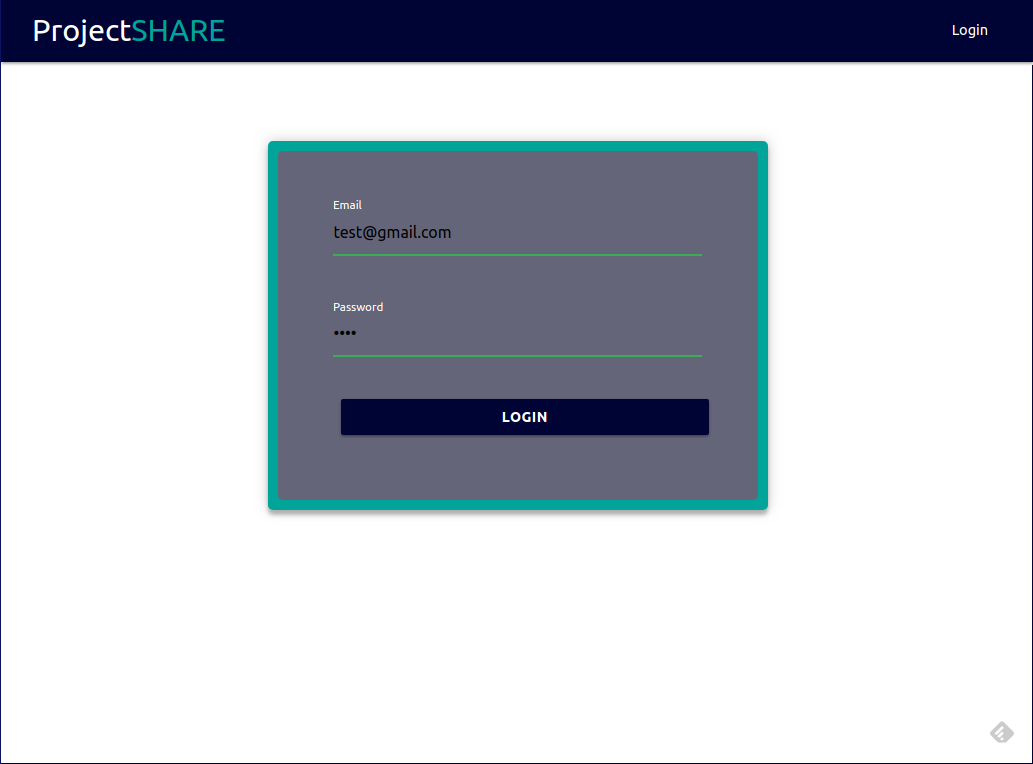
\includegraphics[scale=0.3]{screenLogin}
	}
	\caption{Formularz logowania}
	\centering
\end{figure}


Po zalogowaniu następuje przekierowanie na główny panel z projektami. Jest to widok zawierający 5 najbardziej polecanych projektów dla danego użytkownika, wybranych przez system rekomendacji. Użytkownik aplikacji może przeczytać skrócony opis danego projektu, powiększyć zdjęcie go reprezentujące oraz przejść do rozszerzonego opisu projektu. Od momentu zalogowania, po lewej stronie umieszczona została lista z projektami obserwowanymi, na której widać nazwy wraz ze zdjęciami. Po kliknięciu na dany projekt wysuwa się krótkie zdanie opisujące oraz przekierowanie do rozszerzonego opisu. Jest on zawsze dostępny tak, aby spełnić wymagania klienta i szybkim dostępie do projektów obserwowanych.

\begin{figure}[h!]
	\makebox[\textwidth][c]{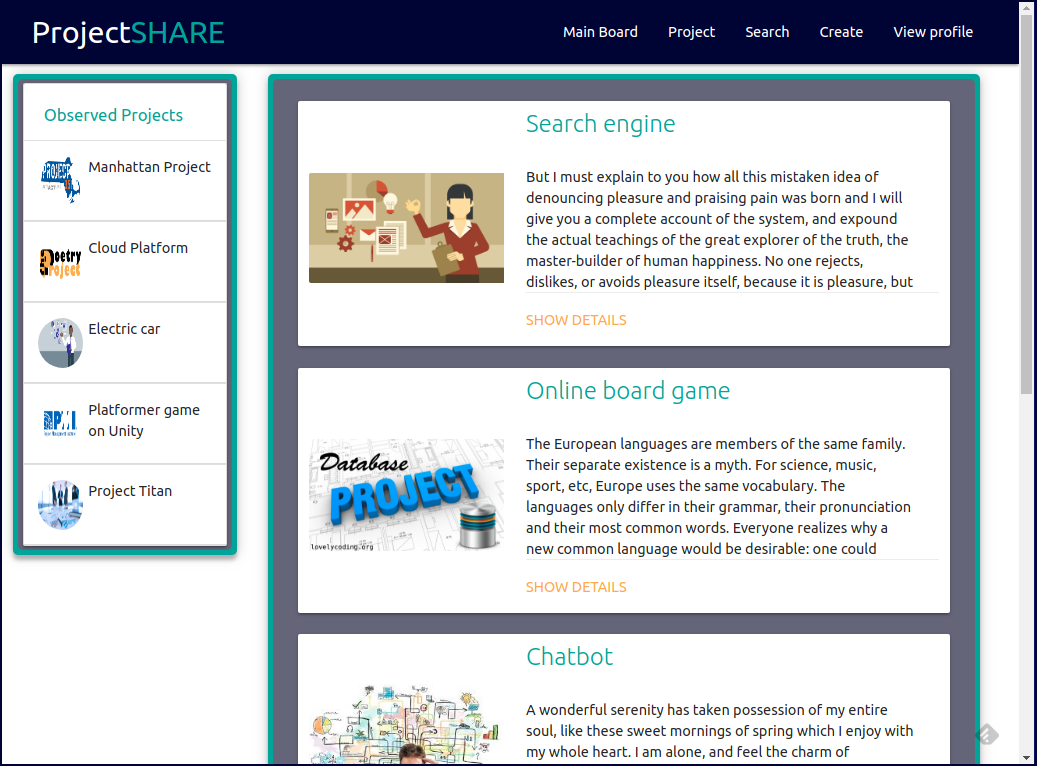
\includegraphics[scale=0.35]{screenMainBoard}
	}
	\caption{Widok z polecanymi projektami}
	\centering
\end{figure}

Kolejnym panelem jest widok rozszerzonego opisu projektu. W pierwszej kolejności przedstawiony jest tytuł, zdjęcie oraz dwa przyciski \textit{subscribe/unsubscribe}, \textit{join/resign}. Za pomocą pierwszego przycisku możemy dodać lub usunąć projekt do listy obserwowanych, a za pomocą drugiego możemy dołączyć do projektu albo z niego zrezygnować. Poniżej znajduje się tekstowy opis ograniczony do 1024 znaków oraz lista zawierająca szczegóły. Następnie wyświetlana jest karta linków związanych z projektem, lista uczestników oraz tagi, którymi dany projekt jest oznaczony.

\begin{figure}[h!]
	\makebox[\textwidth][c]{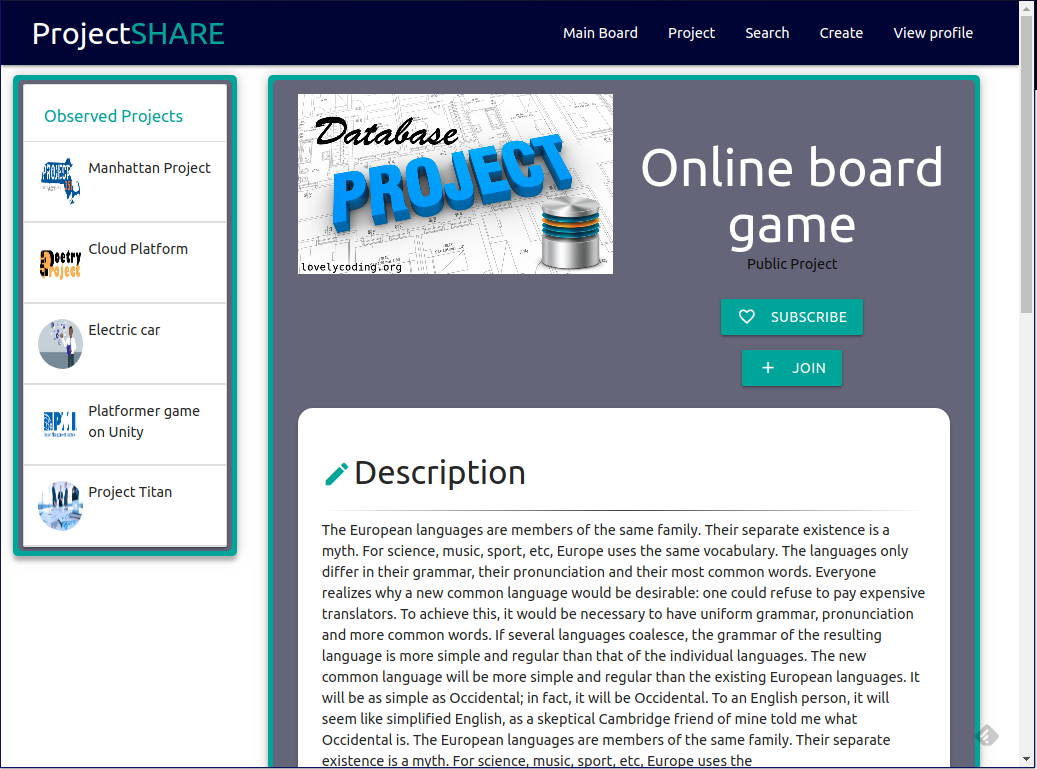
\includegraphics[scale=0.35]{screenProject1}
	}
	\caption{Widok rozszerzonego opisu projektu cz.1}
	\centering
\end{figure}

\begin{figure}[h!]
	\makebox[\textwidth][c]{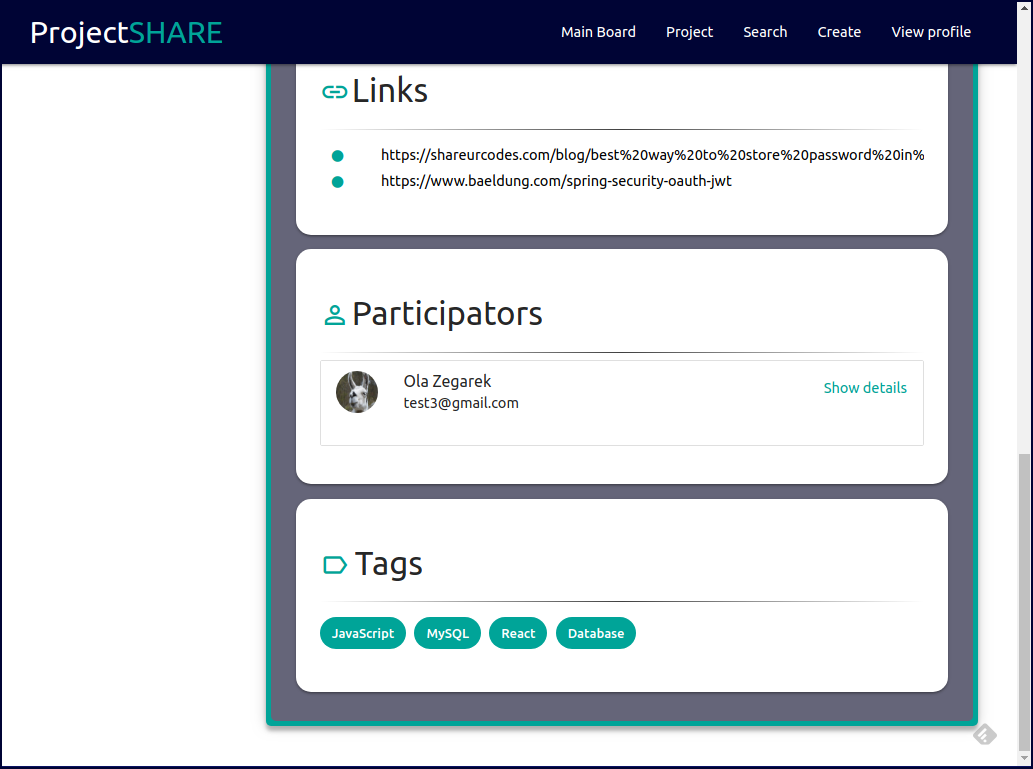
\includegraphics[scale=0.35]{screenProject2}
	}
	\caption{Widok rozszerzonego opisu projektu cz.2}
	\centering
\end{figure}

\bigskip
\bigskip
\bigskip
\bigskip
\bigskip
\bigskip
\bigskip
\bigskip
\bigskip
\bigskip
\bigskip
\bigskip
\bigskip
\bigskip
\bigskip
\bigskip

Kolejnym elementem aplikacji jest widok wyszukiwarki projektów. Podając nazwę można wyszukać podobne inicjatywy oraz przefiltrować je na podstawie tagów. Po pomyślnym wyszukaniu wyświetla się lista projektów w formacie podobnym jak przy głównym panelu.



\begin{figure}[h!]
	\makebox[\textwidth][c]{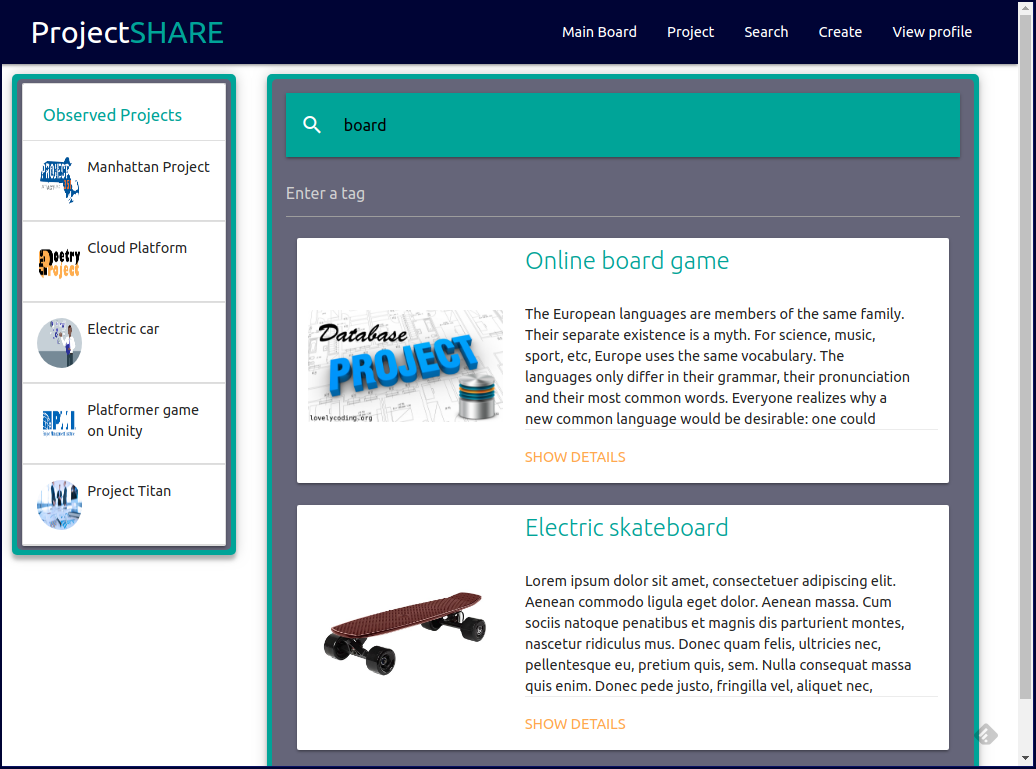
\includegraphics[scale=0.30]{screenSearch}
	}
	\caption{Widok wyszukiwarki projektów}
	\centering
\end{figure}



Do stworzenia projektu został zaprojektowany specjalny widok \textit{CreateProject}. Ułożenie poszczególnych elementów jest podobne jak przy widoku wyświetlania rozszerzonego opisu, ponieważ użytkownik może mieć wtedy wstępne wyobrażenie jaki będzie widok końcowy. Przy tworzeniu projektu należy podać jego nazwę, opis, adres URL do zdjęcia, zaznaczyć czy jest to projekt publiczny czy prywatny, uzupełnić detale, linki oraz oznaczyć go tagami. Po pomyślnym wypełnieniu formularza odblokowany zostaje przycisk \textit{Create}, a użytkownik może stworzyć projekt.

\begin{figure}[h!]
	\makebox[\textwidth][c]{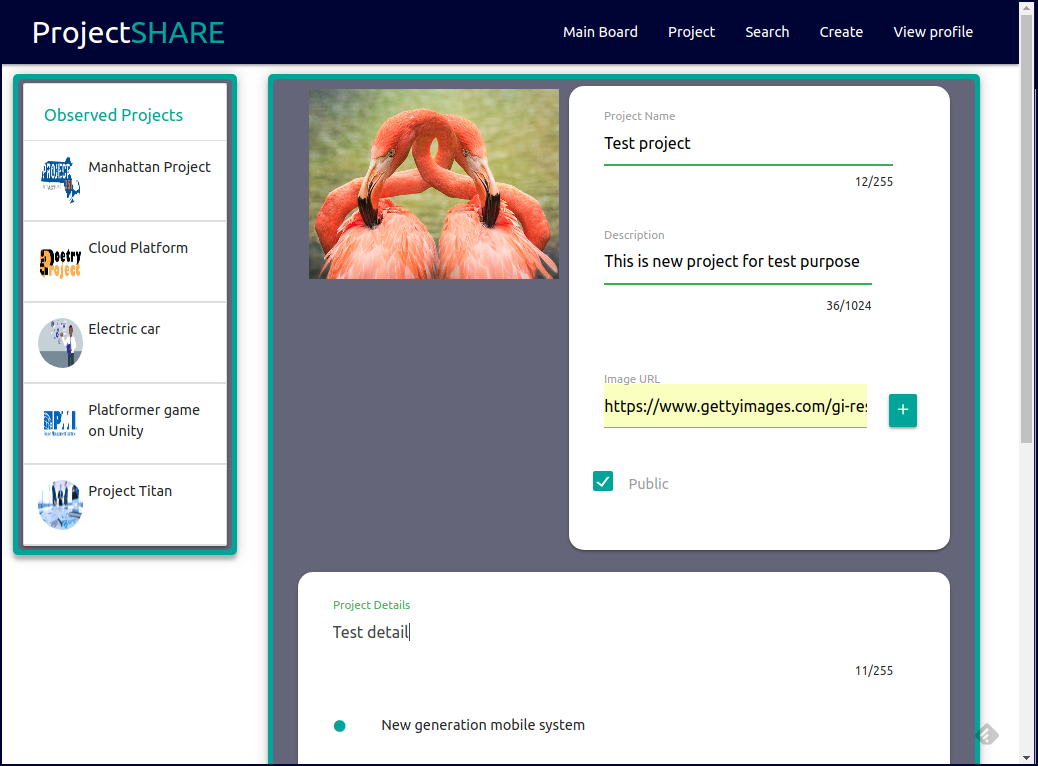
\includegraphics[scale=0.30]{screenCreate1}
	}
	\caption{Widok tworzenia projektu cz.1}
	\centering
\end{figure}

\clearpage

\begin{figure}[h!]
	\makebox[\textwidth][c]{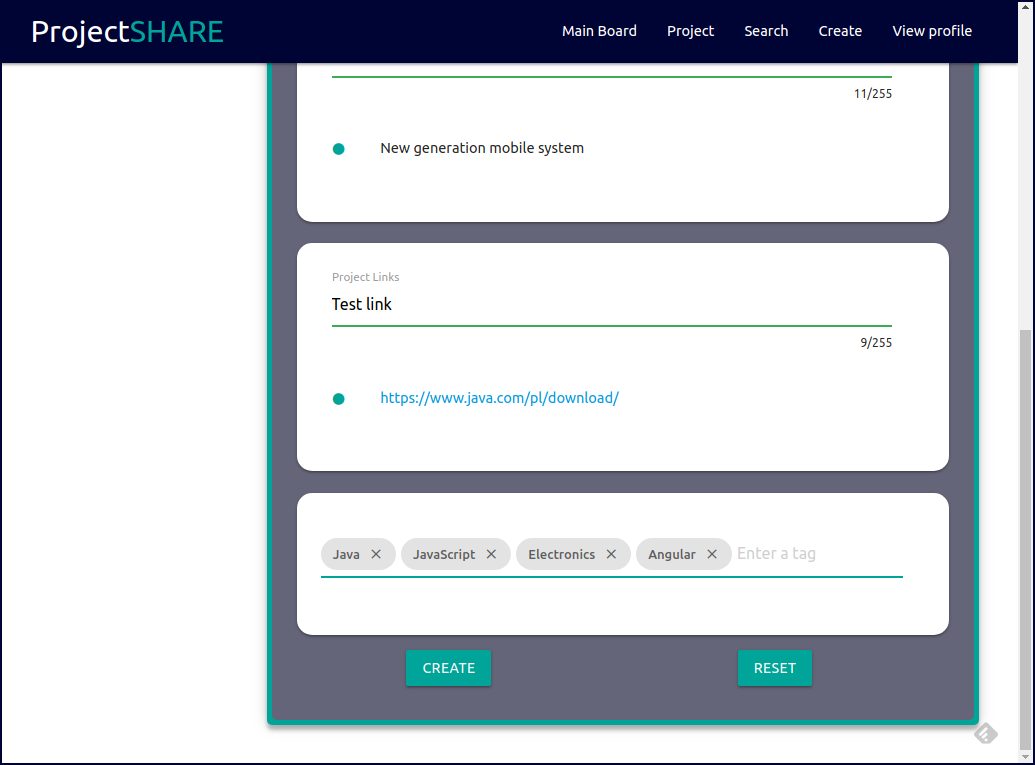
\includegraphics[scale=0.30]{screenCreate2}
	}
	\caption{Widok tworzenia projektu cz.2}
	\centering
\end{figure}


Ostatnim widokiem jest widok użytkownika. Za jego pomocą można sprawdzić z jakiego kraju pochodzi, na jaką uczelnię oraz wydział uczęszczał oraz jaką specjalizacje skończył. Dodatkowo poniżej imienia oraz nazwiska widnieje adres email pozwalający na kontakt z użytkownikiem. Zgodnie z wymaganiami klienta zmieszczono również listę projektów, w których dany użytkownik bierze udział. Ma to na celu zapewnienie możliwości sprawdzenia m.in. czy jest szansa, że będzie On posiadał interesujące informacje, czy posiada odpowiednie kompetencje w danym zakresie.

\begin{figure}[h!]
	\makebox[\textwidth][c]{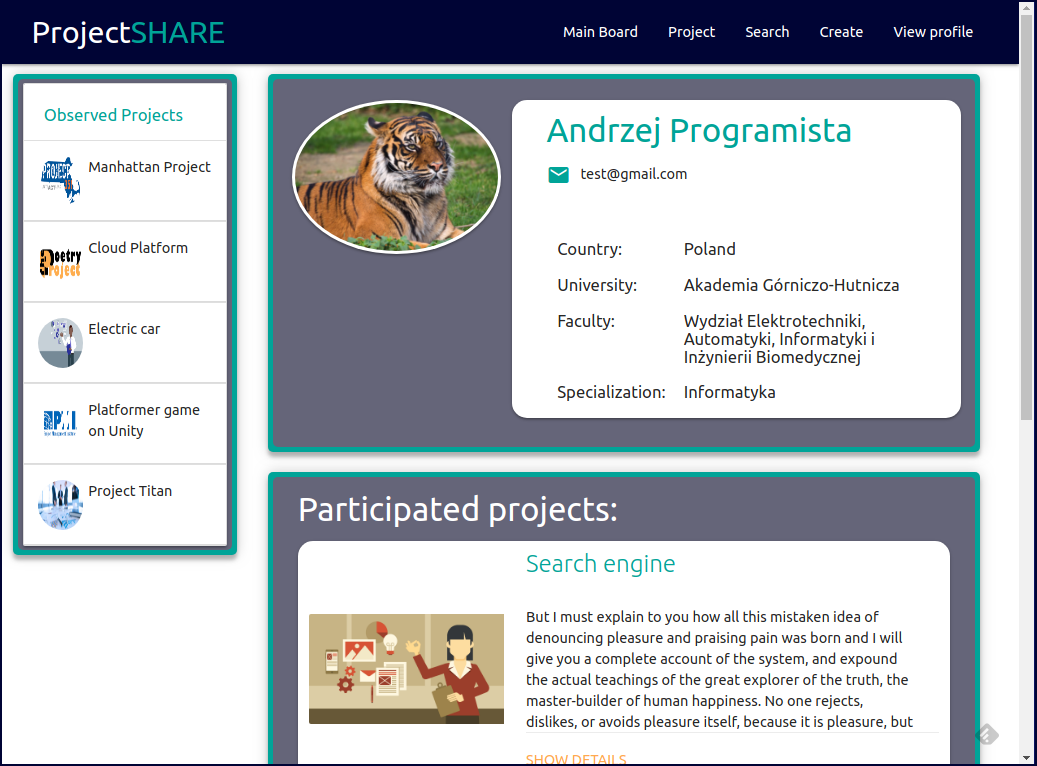
\includegraphics[scale=0.30]{screenUser}
	}
	\caption{Widok z informacjami o użytkowniku}
	\centering
\end{figure}

\clearpage

\section{Implementacja algorytmu rekomendacji}

Do stworzenia systemu rekomendacji wykorzystano opisywany wcześniej algorytm Content-based filtering oraz dostosowano go do dziedziny używanej w aplikacji  \mbox{\textit{ProjectSHARE}}. Algorytm wykorzystuje listę projektów obserwowanych przez użytkownika do stworzenia predykcji jak również tagi, którymi projekt jest opisany. Pozwoliło to na małą modyfikację algorytmu tzn. stworzenie binarnej reprezentacji atrybutów projektu. Aby przedstawić działanie systemu oraz wykonywane obliczenia posłużono się podzbiorem danych testowych w postaci 5 projektów. Wyniki przedstawiono w formie tabeli z odpowiednio opisanymi kolumnami.

Pierwszym krokiem jaki należy wykonać jest stworzenie już wspomnianej binarnej reprezentacji. Następnie obliczono podstawowe dane takie jak liczbę wszystkich atrybutów w projekcie oraz parametr \textit{Tag Frequency}, oznaczający liczbę występowań danego taga we wszystkich rozpatrywanych projektach. Aby obliczyć predykcję wybrano 3 z 5 projektów jako obserwowane. Poniżej zamieszczona jest tabela, w której występowanie taga w projekcie oznaczono za pomocą wartości 1, a jego brak jako 0. Poniżej znajdują się kolumny z wyliczonymi parametrami oraz kolumna \textit{User}, w której oznaczono projekty obserwowane przez użytkownika.   

\begin{figure}[h!]
	\makebox[\textwidth][c]{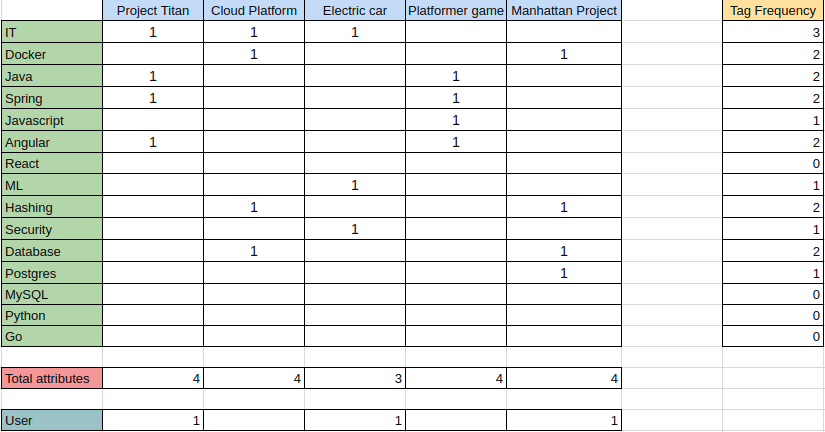
\includegraphics[scale=0.5]{firstStep}
	}
	\caption{Tabele pokazująca wyliczenia powstałe w kroku pierwszym}
	\centering
\end{figure}

Kolejnym krokiem, który wykonano była normalizacja atrybutów poprzez podzielenie ich przez pierwiastek z sumy atrybutów w projekcie. Następnie wykonano obliczenia związane z profilem danego użytkownika. W uproszczeniu oznacza on zainteresowanie użytkownika danym tagiem. Oblicza się go poprzez sumę iloczynów wektora wartości atrybutu po normalizacji dla taga oraz wektora projektów obserwowanych.

\begin{figure}[h!]
	\makebox[\textwidth][c]{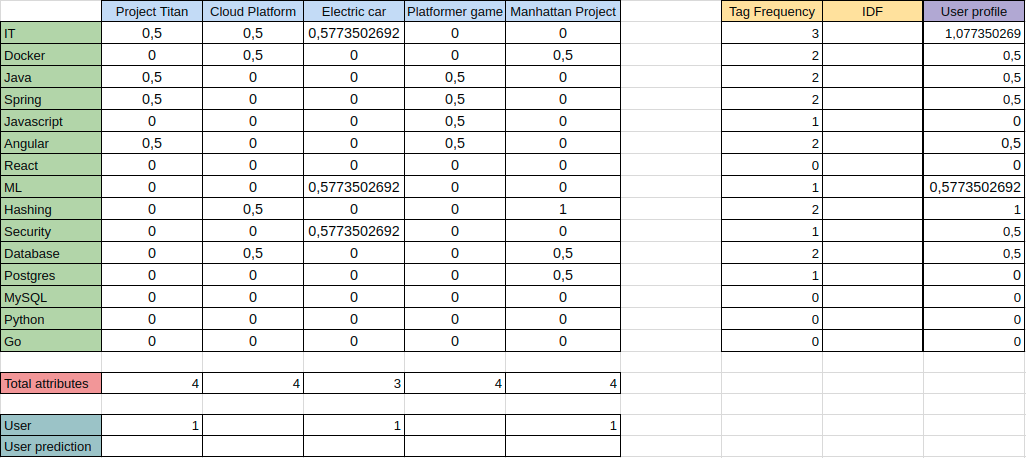
\includegraphics[scale=0.42]{secondStep}
	}
	\caption{Tabele pokazująca wyliczenia powstałe w kroku drugim}
	\centering
\end{figure}

\bigskip
\bigskip

W ostatnim kroku obliczono parametr \textit{Inverse Document Frequency}, którego wartość jest równa logarytmowi dziesiętnemu z liczby wszystkich projektów podzielonej przez liczbę występowań danego taga. Mając już wyliczone wszystkie parametry przystąpiono do przygotowania predykcji dla użytkownika. Obliczono ją poprzez sumę iloczynów wektora wartości atrybutu po normalizacji dla projektu, wektora profilu użytkownika oraz \textit{Inverse Document Frequency}. Na podstawie tak przygotowanej predykcji użytkownikowi wyświetla się pięć projektów z najlepszym wynikiem. 

\begin{figure}[h!]
	\makebox[\textwidth][c]{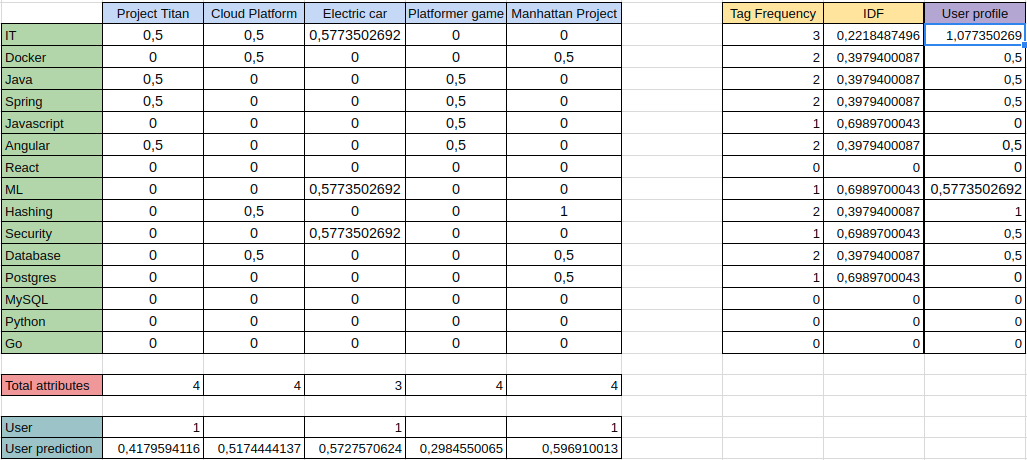
\includegraphics[scale=0.42]{thirdStep}
	}
	\caption{Tabele pokazująca wyliczenia powstałe w kroku trzecim}
	\centering
\end{figure}

\clearpage

\section{Testy systemu rekomendacji}

W celu przetestowania działania systemu rekomendacji w praktyce przygotowano specjalny zestaw danych testowych. Stworzono trzech użytkowników reprezentujących trzy osobne dziedziny zainteresowań: programowanie, mechanika, biologia. Każdy z użytkowników zaobserwował 5 projektów zgodnych z jego zainteresowaniami. Na potrzeby testu stworzono ich łącznie 30, po 10 na każdą przewidzianą dziedzinę. 
Głównym celem testu było sprawdzenie, czy na panelu projektów polecanych pojawią się projekty zgodne z zainteresowaniami danego użytkownika. Dodatkowo porównano za pomocą tabeli tagi projektów obserwowanych oraz polecanych, wraz ze współczynnikiem zgodności danego projektu z zainteresowaniami użytkownika. 


Poniżej umieszczone są wyniki przeprowadzonego testu, postaci tabel porównawczych

\begin{figure}[h!]
	\makebox[\textwidth][c]{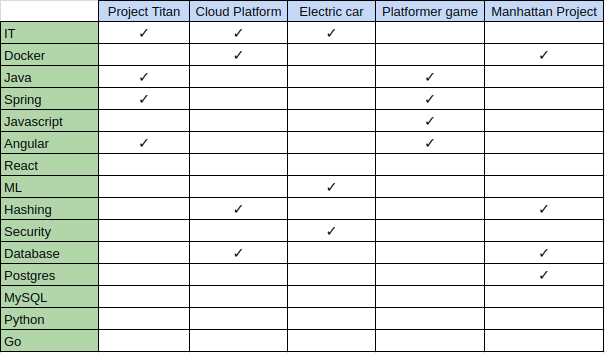
\includegraphics[scale=0.48]{tabelaprog1}
	}
	\caption{Projekty zaobserwowane przez użytkownika o zainteresowaniach programistycznych wraz z tagami}
	\centering
\end{figure}

\begin{figure}[h!]
	\makebox[\textwidth][c]{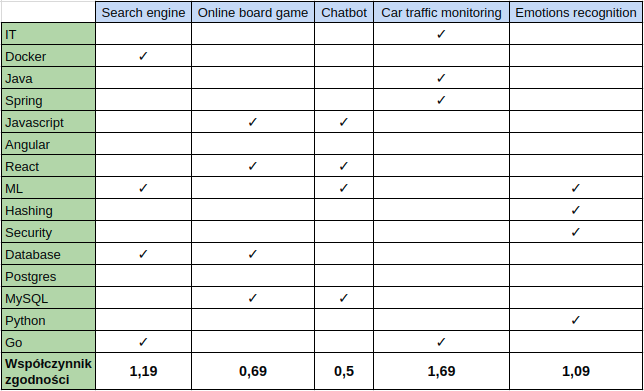
\includegraphics[scale=0.48]{tabelaprog2}
	}
	\caption{Projekty polecone użytkownikowi o zainteresowaniach programistycznych wraz z tagami oraz wyliczonym współczynnikiem zgodności}
	\centering
\end{figure}





\begin{figure}[h!]
	\makebox[\textwidth][c]{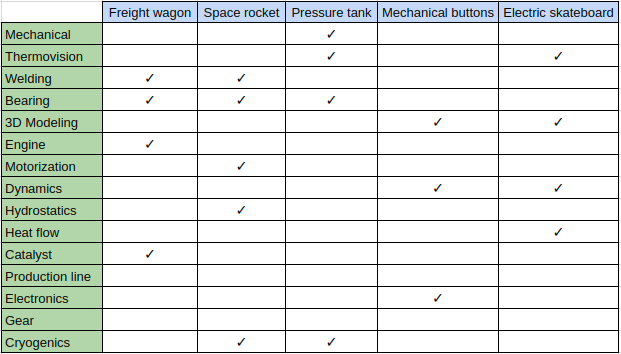
\includegraphics[scale=0.5]{tabelamech1}
	}
	\caption{Projekty zaobserwowane przez użytkownika o zainteresowaniach mechanicznych wraz z tagami}
	\centering
\end{figure}

\begin{figure}[h!]
	\makebox[\textwidth][c]{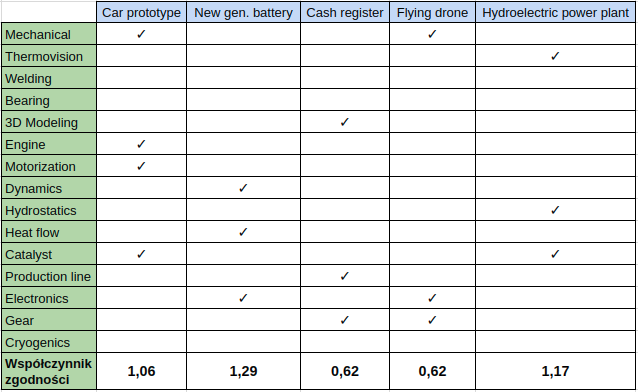
\includegraphics[scale=0.5]{tabelamech2}
	}
	\caption{Projekty polecone użytkownikowi o zainteresowaniach mechanicznych wraz z tagami oraz wyliczonym współczynnikiem zgodności}
	\centering
\end{figure}





\begin{figure}[h!]
	\makebox[\textwidth][c]{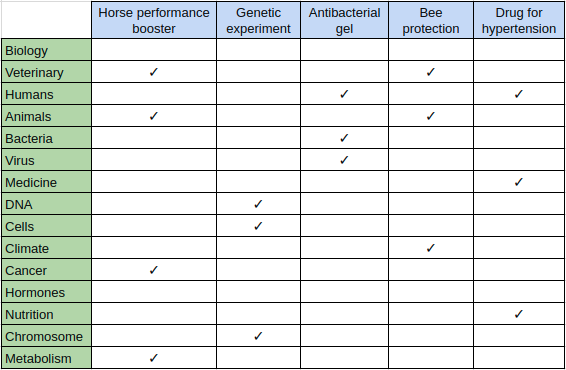
\includegraphics[scale=0.5]{tabelabiol1}
	}
	\caption{Projekty zaobserwowane przez użytkownika o zainteresowaniach biologicznych wraz z tagami}
	\centering
\end{figure}

\begin{figure}[h!]
	\makebox[\textwidth][c]{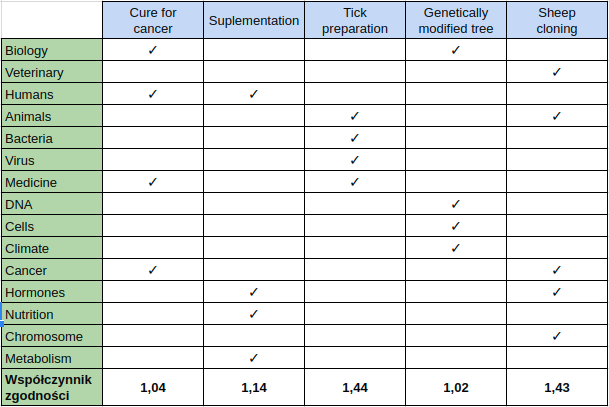
\includegraphics[scale=0.5]{tabelabiol2}
	}
	\caption{Projekty polecone użytkownikowi o zainteresowaniach biologicznych wraz z tagami oraz wyliczonym współczynnikiem zgodności}
	\centering
\end{figure}
